\documentclass[oneside]{article}
\title{Exercise 1}
\author{Orgho Anoronyo Neogi}
\date{09 December 2016}
\usepackage{amsmath}
\usepackage{graphicx}
\usepackage{minted}
\usepackage{float}
\usemintedstyle{emacs}
\usepackage[colorlinks=true]{hyperref}

\newenvironment{answer}
  {\vspace*{0.2cm} \rule{12cm}{0.02cm} \vspace*{0.2cm}}
  {\vspace*{0.2cm}}

\begin{document}
\maketitle

\begin{enumerate}
	\item A function of two variables, each of which takes a value in the interval [0,1], that returns a vector that describes a point on a cylinder (but not on the cylinder's circular end caps).

	      \begin{answer}
	      	\inputminted[firstline=1, lastline=9]{js}{exercise-1.js}
	      \end{answer}

	\item A function of two variables, each of which takes a value in the interval [0,1], that returns a vector that describes a point on a cone (but not on the cone's circular base).

	      \begin{answer}
	      	\inputminted[firstline=11, lastline=19]{js}{exercise-1.js}
	      \end{answer}

	\item A function of two variables, each of which takes a value in the interval [0,1], that returns a vector that describes a point on a sphere.

	      \begin{answer}
	      	\inputminted[firstline=21, lastline=29]{js}{exercise-1.js}
	      \end{answer}

	\item A mathematical expression that describes the brightness of a small patch of a surface. The expression should contain terms that model ambient lighting, diffuse reflection, and specular reflection. It should show the role of a vector that is perpendicular to the surface, a vector that points to the source of light, and a vector that points to the eye of the viewer in the calculation of these several components of the surface's illumination.

	      \begin{answer}
	      	$$I_p = k_a i_a + \sum_{m\in lights} (k_d (\hat{L}_m \cdot \hat{N}) i_{m,d} + k_s (\hat{R}_m \cdot \hat{V})^{\alpha}i_{m,s})$$

	      	$k_s$ is specular reflection constant.

	      	$k_d$ is diffuse reflection constant.

	      	$k_a$ is  ambient reflection constant.

	      	$\alpha$ is ''shininess'' constant for this material

	      	$lights$ is the set of all light sources

	      	$\hat{L}_m$ is the direction vector from the point to light source specified by $m$

	      	$\hat{N}$ is the normal vector

	      	$\hat{R}_m$ is the direction of a perfectly reflected ray of light

	      	$\hat{V}$ is the direction towards the viewer
	      \end{answer}

	\item A mathematical expression that describes a point on a cubic B\'{e}zier curve as a product of vector(s) and matrice(s).

	      \begin{answer}
	      	\begin{align*}
	      		\begin{matrix}
	      		\begin{bmatrix}
	      		1  & t  & t^2 & t^3
	      		\end{bmatrix} \\
	      		\mbox{} \\
	      		\mbox{} \\
	      		\mbox{}
	      		\end{matrix}
	      		\begin{bmatrix}
	      		  & 1  & 0  & 0  & 0 \\
	      		  & -3 & 3  & 0  & 0 \\
	      		  & 3  & -6 & 3  & 0 \\
	      		  & -1 & 3  & -3 & 1
	      		\end{bmatrix}
	      		\begin{bmatrix}
	      		p_0 \\
	      		p_1 \\
	      		p_2 \\
	      		p_3
	      		\end{bmatrix}
	      		& = P(t)
	      	\end{align*}

	      	Where $p_0, p_1, p_2$ and $p_3$ are the 4 control points
	      \end{answer}

	\item A matrix that describes a perspective transformation.

	      \begin{answer}
	      	\begin{align*}
	      		\begin{bmatrix}
	      		  & \frac{2n}{r-l} & 0              & \frac{r+l}{r-l}  & 0                \\
	      		  & 0              & \frac{2n}{t-b} & \frac{t+b}{t-b}  & 0                \\
	      		  & 0              & 0              & -\frac{f+n}{f-n} & -\frac{2fn}{f-n} \\
	      		  & 0              & 0              & -1               & 0
	      		\end{bmatrix}
	      	\end{align*}

	      	Where $f$ stands for far value, $n$ stands for near value, $t$ stands for top, $b$ stands for bottom, $r$ stands for left and $l$ stands for right.
	      \end{answer}

	\item An image from a program that you write. This program will produce an image of one of the American manned spacecraft of the 1960s and 1970s. Begin by modelling a vehicle with cylinders and cones, then elaborate. Add more details to the vehicle, a background that might include planets and stars, or add animation.

	      \begin{answer}

	      	See this image~\ref{rocket}:

	      \end{answer}

	\item An excerpt from your program that shows us some key feature of the program. This might be a loop, the definition of a function, a call to a function, an assignment state that contains on its right hand side a key expression, or something else.

	      \begin{answer}
	      	\inputminted[firstline=31, lastline=55]{js}{spaceship/scripts/main.js}
	      \end{answer}


	      \begin{figure}[b!]
	      	\begin{center}
	      		\label{rocket}
	      		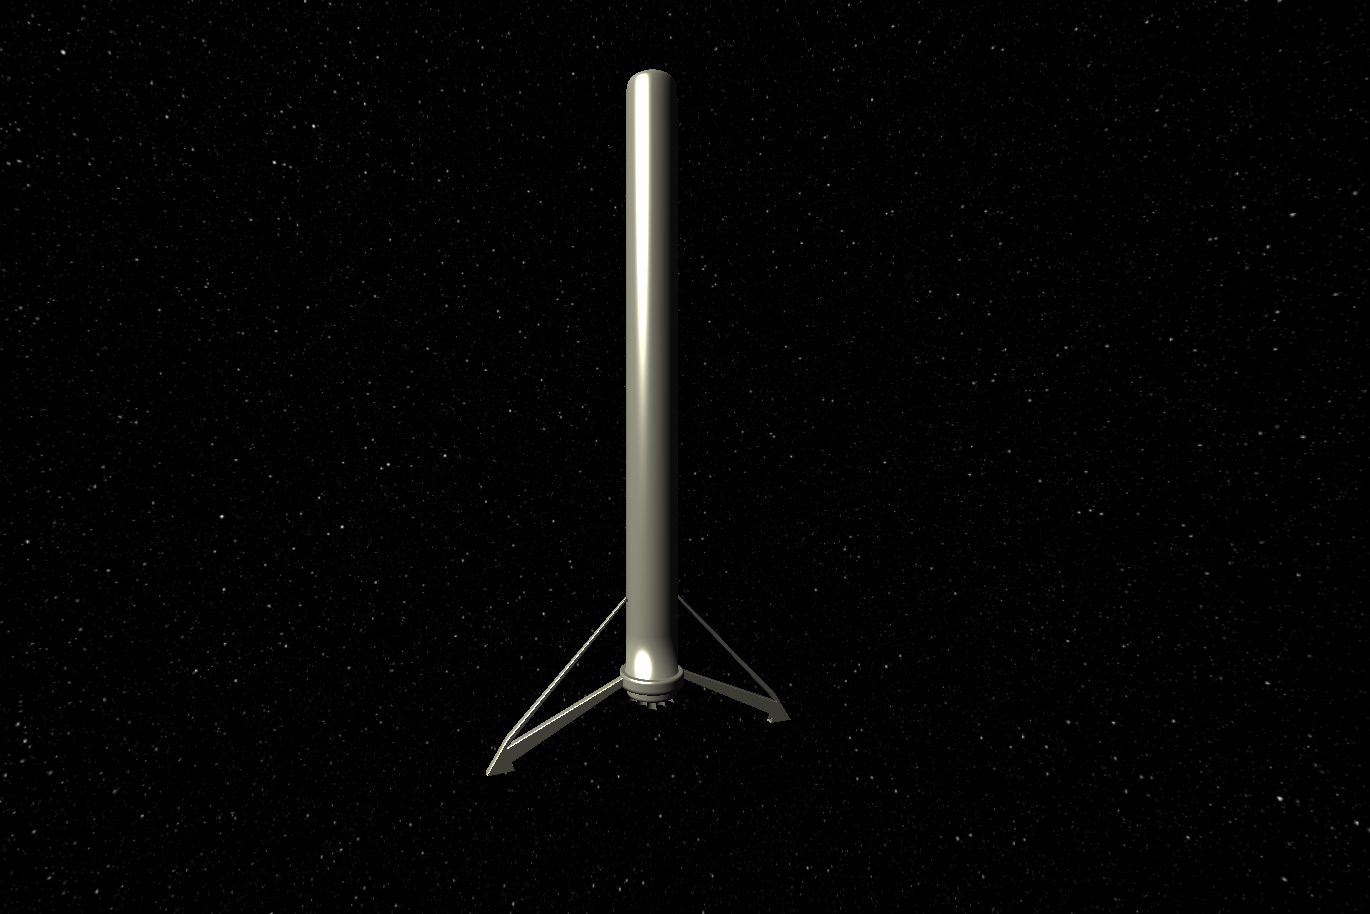
\includegraphics[width=\linewidth]{shitty-rocket}
	      	\end{center}
	      	\caption{Rocket}
	      \end{figure}

\end{enumerate}

\end{document}
